\section{Methodology}
\ac{CUPID}, a new method developed for pure shift \ac{NMR}, fits into the category
of techniques which utilise \ac{2DJ} estimation. In this section, a description
of it is given.

\subsection{The Estimation Routine}
Recall the assumption that a \ac{2DJ} \ac{FID} takes the functional form
of \cref{eq:jres-fid}. The primary steps involved in estimating a \ac{2DJ}
dataset, for a given spectral region of interest, are:
\begin{enumerate}
    \item Generation of a frequency-filtered sub-\ac{FID} corresponding to
        the region of interest (\textit{vide infra}:
        \cref{subsec:jres-filtering}).
    \item Prediction of the sub-\ac{FID}'s model order, either by applying the
        \ac{MDL} on the first increment in the direct dimension\footnote{
            The first increment of a \ac{2DJ} experiment, for which $\tone =
            \qty{0}{\second}$, effectively takes the same form as an \ac{FID}
            derived from a pulse-acquire experiment.
        }(\cref{subsec:model-order}) or
        by manually specifying a
        value.
    \item Generation of an initial parameter estimate using the \ac{MMEMPM}
        (\cref{subsec:mmempm}).
    \item Subjection of the initial parameter estimate to phase
        variance-regularised \ac{NLP} (\cref{sec:nlp}).
\end{enumerate}
Instead of estimating successive \ac{1D} \acp{FID}, as proposed by
Nuzillard and Mutzenhardt et al., \ac{2DJ} sub-\acp{FID} are considered
holistically; a number of benefits are realised because of this.
First, multiplet structures which heavily overlap in a
conventional \ac{1D} dataset can become separated in the \ac{2DJ} dataset,
assuming that the Larmor frequencies of the relevant spins are sufficiently
different.
Accurate resolution of the \ac{FID}'s constituent signals in more crowded spectral
regions is far more likely to be successful with a full \ac{2D} estimation as a
result.
On top of this, there is an additional resolution advantage relative to the
estimation of \emph{direct} dimension \ac{1D} \acp{FID}. Due to the presence of a spin
echo during $\tone$, signal damping effects caused by field inhomogeneities are
nullified, such that damping is dictated solely by transverse relaxation
($T_2^{\vphantom{*}}$). During $\ttwo$ however, the influence of field inhomogeneities are not
corrected, such that damping occurs at a faster rate, characterised by $T_2^*$
(see \cref{fn:t2-star} in \cref{sec:seq}).
As such, multiplet structures in the indirect dimension exhibit better
resolution (assuming $\nicefrac{\fswone}{\None}$ and
$\nicefrac{\fswtwo}{\Ntwo}$ are comparable).
A further benefit comes with having access to the frequencies of
signals in \emph{both} dimensions, since this opens up the opportunity to group
together those which belong to the same multiplet, as will be discussed in
\cref{subsec:mp-selection}.
Similar information can be obtained
by extracting cross-sections of a sheared magnitude-mode \ac{2DJ} spectrum at
appropriate values of $F^{(2)}$, though the lineshapes of peaks suffer from the
undesirable characteristics described above. The
\ac{ZS}-\ac{2DJ}\cite{Pell2007} and
\ac{PSYCHE}-\ac{2DJ}\cite{Foroozandeh2015,Kiraly2017} experiments are also able
to generate individual multiplet structures, though with long \ac{3D} pulse
sequences, and with reduced sensitivity relative to a conventional \ac{2DJ}
experiment.

As was mentioned in \cref{subsec:model-order}, application of the
\ac{MDL} on a \ac{2D} \ac{FID} is not desirable, since a complete \ac{SVD}
computation would need to be undertaken on the typically very large
block-Hankel matrix $\symbf{E}_{\symbf{Y}}$.
Assuming that the spectral region being considered is not too
crowded, applying the \ac{MDL} on the first direct-dimension \ac{FID} can
return reasonable estimates of $M$ at a far smaller computational cost. For
particularly crowded regions, resorting to a manual specification of model
order by inspecting the \ac{2DJ} spectrum is the best solution currently
available.
An interesting benefit is sometimes realised when the \ac{1D} \ac{MDL} is
used for model order selection.
The presence of strong coupling artefacts leads to
additional nuisance peaks featuring in spectra produced by the
shear-and-project approach. Exactly the
same phenomenon would occur when estimation is employed, assuming
that the strong coupling artefacts are incorporated into the parameter
set. However, since the
artefacts have direct-dimension frequencies which are identical to those of
first-order signals in the dataset, it is incredibly challenging to resolve
these using the \ac{1D} \ac{MDL} approach. Therefore, the \ac{MDL} is often
found to predict a model order which agrees with the number of first-order
signals, rather than the \emph{true} number of signals in the \ac{FID}. As the
\ac{MMEMPM} generates a parameter estimate based on the first $M$ significant
components of the dataset, the more intense first-order signals are expected to
be quantified, whereas the weaker strong coupling artefacts will be neglected.
It should be noted that this concept is not infallible; it has simply been
observed on a number of occasions. There are instances where strong coupling
artefacts are incorporated into the estimation result, either because the
prediction of $M$ was excessive, or certain artefacts possess particularly
large amplitudes; example of these situations will be given later.

\subsection{The \ang{-45} Signal}
\begin{figure}
    \centering
    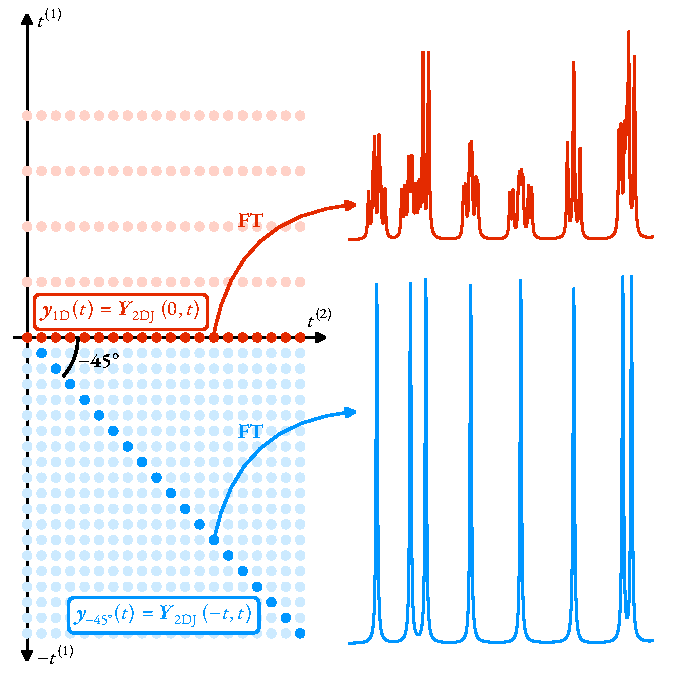
\includegraphics{neg_45_signal/neg_45_signal.pdf}
    \caption[
        An illustration of the reasoning behind the name ``\ang{-45}
        signal'', which is used to generate pure shift spectra as part of
        \acs{CUPID}.
    ]{
        An illustration of the reasoning behind the name ``\ang{-45}
        signal'', which is used to generate pure shift spectra as part of
        \ac{CUPID}. The pale red
        dots denote
        a typical \ac{2DJ} \ac{FID}, where
        the amount and rate of sampling in the direct dimension is greater than
        in the indirect dimension (i.e. $\None \ll \Ntwo$ and $\fswone \ll
        \fswtwo$). The bright red dots correspond to the first direct-dimension
        signal $y_{\text{2DJ}}(0,\ttwo)$, which has the same form as
        \iac{FID} from a pulse-acquire experiment. A hypothetical signal
        generated by propagating the \ac{FID} into $-\tone$, with the same rate
        of sampling in both dimensions, is denoted with pale blue dots. Taking
        the diagonal of this signal, such that it forms a \ang{-45} angle with the
        $\ttwo$ axis\,---\,the convention of angles being defined through an
        anticlockwise rotation starting on the $\ttwo$-axis has been applied
        here\,---\,yields an \ac{FID}
        $\by_{\ang{-45}}$  which is
        homodecoupled. Note that there is a slight discrepancy
        between \cref{eq:neg-45} and this description, in that the
        indirect dimension damping factors $\bdetaone$ are neglected in the
        former case.
    }
    \label{fig:neg-45}
\end{figure}
The \ac{2DJ} estimation routine yields the parameter vector $\bth \in
\mathbb{R}^{6M}$. With
knowledge of the frequencies and damping factors in both dimensions, it is
possible to generate \iac{FID} which will produce a pure shift spectrum
directly, rather proceeding via the full-echo approach of Nuzillard and
Mutzenhardt et al.
The desired synthetic \ac{FID} produced is named the \emph{\ang{-45} signal}
$\symbf{y}_{\ang{-45}} \in \mathbb{C}^{\Ntwo}$:
\begin{equation}
    y_{\ang{-45},\ntwo} =
        \sum_{m=1}^{M} a_m \exp (\iu \phi_m)
        \exp\left(\left(2 \pi \iu \left(\ftwo_m - \fone_m - \foff\right)
                - \etatwo_m
            \right) \ntwo \Dttwo
        \right),
    \label{eq:neg-45}
\end{equation}
with the reasoning behind the name provided by \cref{fig:neg-45}.
The \ang{-45} signal
takes the form of a conventional \ac{1D} \ac{FID},
except that the frequency of each oscillator, which would be $\ftwo_m$ in a
pulse-acquire experiment,
is replaced with $\ftwo_m - \fone_m$. Oscillators belonging to the same
multiplet $s$ will all provide a contribution to the \ac{FID} with the
angular frequency $\omega_{0,s}$.
Assuming that the parameters associated with the \ac{2DJ}
\ac{FID} are accurately determined, a pure shift spectrum with sharp
absorption-mode lineshapes and no loss of signal can be generated by
constructing the \ang{-45} signal.


\subsection{Filtration of \ac{2DJ} Data}
\label{subsec:jres-filtering}
Unlike the direct dimension, which can often comprise sparsely distributed
peaks in the Fourier domain, the indirect dimension of \ac{2DJ} datasets tends
to be densely populated since all multiplet structures are centered at
\qty{0}{\hertz}, and rarely span beyond $\pm \qty{50}{\hertz}$. As such,
the generation of frequency-filtered sub-\acp{FID} is limited to
the direct dimension in \ac{CUPID}.
The filtering procedure applied to \ac{2DJ} data is an extension of that
for \ac{1D} data described in \cref{sec:filtering}:
\begin{enumerate}
    \item The array $\symbf{Y}_{\text{VE}} \in \mathbb{C}^{\None \times 2
        \Ntwo}$, is constructed, which contains the \ac{VE} of each
        direct-dimension \ac{FID}, i.e. each row of the array is given by
        \begin{equation}
            \begin{gathered}
            \by_{\text{VE},\none} =
                \begin{bmatrix}
                    \Re\left(y_{n^{(1)}, 0}^{\vphantom{*}}\right) &
                    y_{n^{(1)}, 1}^{\vphantom{*}} &
                    \cdots &
                    y_{n^{(1)}, \Ntwo - 1}^{\vphantom{*}} &
                    0 &
                    y_{n^{(1)}, \Ntwo - 1}^* &
                    \cdots &
                    y_{n^{(1)}, 1}^*
                \end{bmatrix},\\
                \forall n^{(1)} \in \lbrace 0, \cdots, N^{(1)} - 1 \rbrace.
            \end{gathered}
        \end{equation}
    \item $\symbf{Y}_{\text{VE}}$ is subjected to \ac{FT} along the direct
        dimension to produce the spectrum  $\symbf{S}_{\text{VE}}$
        (\cref{fig:jres-filtering}.a); this has an imaginary component of
        zeros.
    \item A super-Gaussian $\symbf{G} \in \mathbb{R}^{\None \times 2 \Ntwo}$ is
        constructed
        (\cref{fig:jres-filtering}.b):
        \begin{equation}
            \symbf{G} = \symbf{1} \otimes \symbf{g}^{(2)},
        \end{equation}
        where $\symbf{1} \in \mathbb{R}^{\None}$ is a vector of ones, and
        $\symbf{g}^{(2)} \in \mathbb{R}^{2\Ntwo}$ is a super-Gaussian vector
        given by \cref{eq:super-Gaussian-onedim}.
    \item A matrix of additive noise is generated by extracting the variance
        $\sigma^2$ of a direct-dimension strip of $\symbf{S}_{\text{VE}}$ which
        is devoid of peaks, and generating an array $\symbf{W}_{\sigma^2} \in
        \mathbb{R}^{\None \times 2 \Ntwo}$ with values independently sampled
        from $\mathcal{N}(0, \sigma^2)$ (\cref{fig:jres-filtering}.c).
    \item The spectrum is filtered (\cref{fig:jres-filtering}.d):
        \begin{equation}
            \widetilde{\symbf{S}}_{\text{VE}} = \symbf{S}_{\text{VE}} \odot
            \symbf{G} + \symbf{W}_{\sigma^2} \odot (\symbf{1} - \symbf{G}).
        \end{equation}
    \item $\widetilde{\symbf{S}}_{\text{VE}}$ is subjected to \ac{IFT} and is
        sliced in half in the direct dimension, yeilding the final filtered
        signal $\widetilde{\symbf{Y}}$.
\end{enumerate}
As with the \ac{1D} case, this method can also be extended to
incorporate spectral slicing, acting to reduce the number of points present in
the filtered sub-\ac{FID}.

\begin{figure}
    \centering
    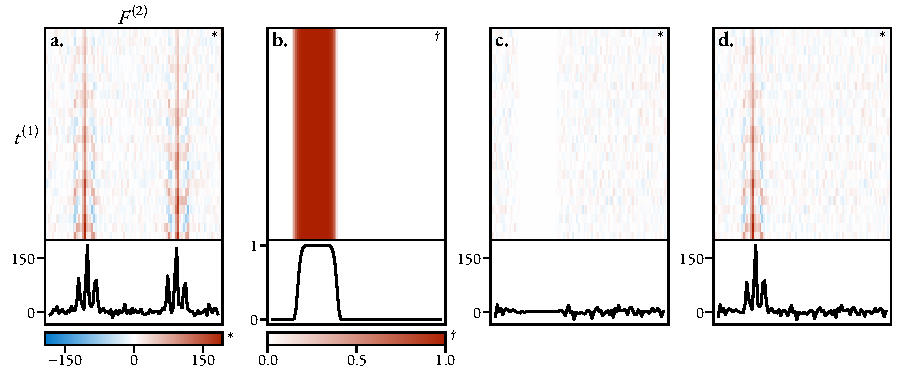
\includegraphics{jres_filtering/jres_filtering.pdf}
    \caption[
        An illustration of the filtering procedure for \acs{2DJ} data.
    ]
    {
        An illustration of the filtering procedure for \ac{2DJ} data.
        Each panel consists of a heat-map of the complete \ac{2D} array, as well as
        a plot of the first slice of the array in the direct dimension ($x$-axis).
        \textbf{a.} The spectrum $\symbf{S}_{\text{VE}}$,
        \textbf{b.} Super-Gaussian filter $\symbf{G}$,
        \textbf{c.} Additive noise, attenuated by the super-Gaussian, $\symbf{W}_{\sigma^2} \odot (\symbf{1} - \symbf{G})$,
        \textbf{d.} Filtered spectrum $\widetilde{\symbf{S}}_{\text{VE}}$
        Figures \ref{fig:jres-filtering}.a to \ref{fig:jres-filtering}.d
        are analogous to
        Figures \ref{fig:jres-filtering}.b to \ref{fig:jres-filtering}.e
        for the \ac{1D} case.
    }
    \label{fig:jres-filtering}
\end{figure}


\subsection{Multiplet Prediction}
\label{subsec:mp-selection}
\ac{CUPID}'s ability to group oscillators present in a parameter set into
multiplet structures relies on simultaneously knowing both the indirect- and
direct-dimension frequencies of each model oscillator. As has already been
established, for oscillators which are associated with the same multiplet
grouping $G_s$, the quantities $\ftwo_{m_1} - \fone_{m_1}$ and $\ftwo_{m_2} -
\fone_{m_2}$ should be equal ($\omega_{0,s}$) for any pairing  $m_1, m_2 \in
G_s$. An assessment of whether two oscillators belong to the same multiplet can
therefore be made using the following criterion:
\begin{equation}
    \left \lvert
        \left( \ftwo_{m_1} - \fone_{m_1} \right) -
        \left( \ftwo_{m_2} - \fone_{m_2} \right)
    \right \rvert < \epsilon.
\end{equation}
$\epsilon \in \mathbb{R}_{>0}$ is a threshold to account for uncertainty in
the estimation result. A lower bound on $\epsilon$ is the separation between
adjacent points in the better-resolved dimension of the spectrum, i.e.
$\min\left(\nicefrac{\fswone}{\None},
\nicefrac{\fswtwo}{\Ntwo}\right)$.  However, limitations in resolution due to
relaxation-induced signal damping and field inhomogeneities can require
$\epsilon$ to be increased beyond this for effective assignments
to be achieved. \Cref{lst:mp-assign} provides a \Python routine that
can be used for multiplet prediction.

There are certain circumstances where it is safe to assume that a
particular oscillator in the estimation result is not associated with a
first-order signal in the dataset;
no oscillator which was derived from a first-order signal will abide by both of
the following:
\begin{enumerate}
    \item The oscillator is not grouped with any other oscillator as part of
        the multiplet assignment.
    \item The magnitude of the indirect dimension frequency of the oscillator
        is appreciably greater than \qty{0}{\hertz}.
\end{enumerate}
If a first-order signal is the only
member of a multiplet grouping, it must be a singlet, and as such it will have
an indirect-dimension frequency of \qty{0}{\hertz}. Oscillators which do agree
with the two points above can be assumed to be related to either strong
coupling artefacts or noise, and can be automatically discarded from the final
parameter estimate.
